\documentclass[journal,12pt,twocolumn]{IEEEtran}
\usepackage{tkz-euclide} % loads TikZ and tkz-base
\usepackage{hyperref}
\usepackage{xcolor}
\title{
\textbf {REPORT ON SOFTWARE PROJECT}\\ \large \textbf{AI1110}: Probability and Random Variables\\Indian Institute of Techonology Hyderabad
}
\author{SURBHI\\CS22BTECH11057}

\begin{document}

\maketitle

\section{Introduction}
The Music Player project is a simple application that allows users to play and control the playback of audio files. This project is implemented using the Pygame library in Python, which provides functionality for graphics and audio. The application provides basic functionalities such as playing the next or previous song, pausing and resuming the playback, and displaying the currently playing song.The provided code is a simple music player implemented using the Pygame library. It allows users to play a shuffled playlist of 20 songs and provides basic controls through a graphical user interface (GUI).

\section{Implementation}
Playlist Creation:\\
The code starts by creating a list of audio files representing the songs in the playlist.The create\_random\_playlist function shuffles the list to create a random order for the songs.\\

Music Playback:\\
The Pygame library is initialized using pygame.init().The code loops through each song in the random playlist.For each song, it loads the audio file using pygame.mixer.music.load(song) and plays it using pygame.mixer.music.play().The code then waits until the song finishes playing using pygame.mixer.music.get\_busy() in a while loop.After the song finishes, the previous song is stopped using pygame.mixer.music.stop().\\

Graphical User Interface (GUI):\\
The GUI window is titled "Music Player" using pygame.display.set\_caption.It defines the font for the buttons and creates rectangles for the start, pause, and next button.It checks for key presses to control the music playback:Pressing the spacebar starts or pauses the current song.\\
Pressing the right arrow key plays the next song in the playlist.\\

Clean-Up:\\
After the main loop ends, the pygame mixer is cleaned up using pygame.mixer.quit().

\begin{itemize}
\item Importing necessary libraries and initializing pygame.
\item Defining color constants using pygame's Color class.
\item Creating the pygame screen and initializing the mixer for audio playback.
\item Defining a Button class to represent the control buttons in the music player.
\item Setting up the initial song list and play stack.
\item Creating instances of the Button class for previous, next, and play buttons.
\item Setting up the main loop to handle events and update the screen.
\item Handling button clicks and updating the play stack accordingly.
\item Loading and playing the selected song using pygame's mixer.
\end{itemize}

\subsection{Dependencies}
To run the Music Player, the following dependencies are required:

\begin{itemize}
\item Python 
\item pygame library
\item random 
\end{itemize}

Additionally, the following modules are used:

\begin{itemize}
        \item os
\end{itemize}

\section{Conclusion}
The Music Player project provides a basic music player application with features such as playing audio files, controlling playback, and displaying the currently playing song. It demonstrates the use of Pygame and its audio capabilities in Python programming.

\begin{figure}
    \centering
    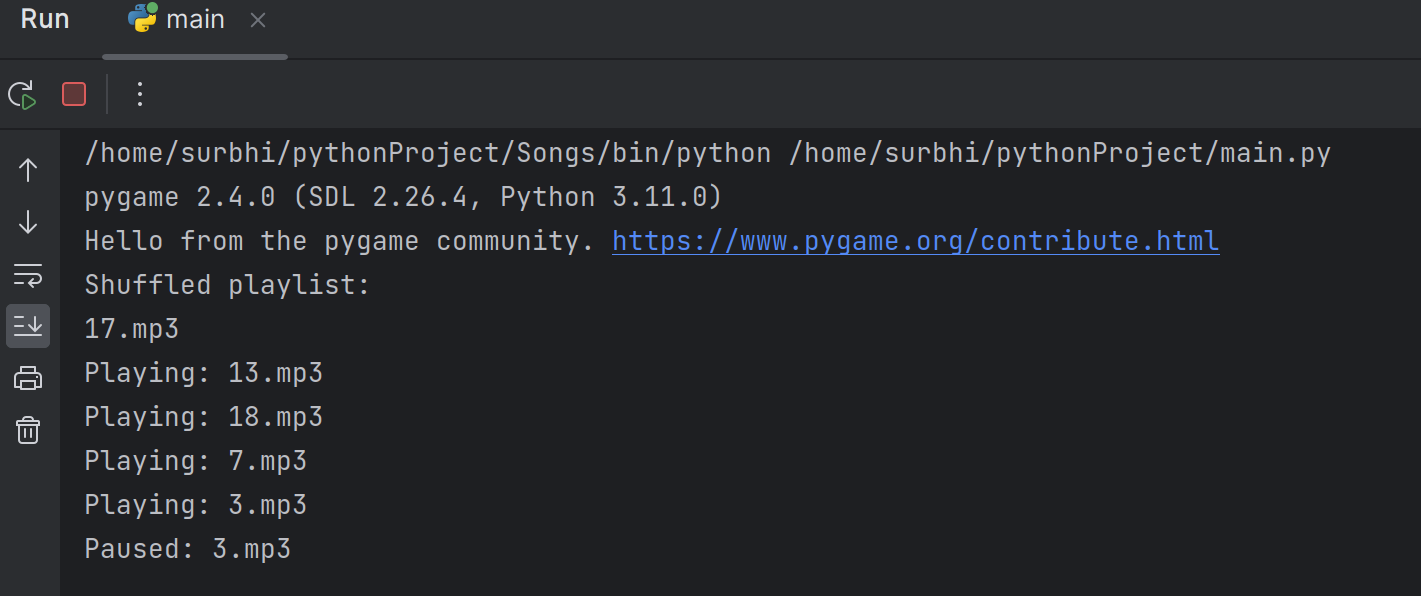
\includegraphics[width=\linewidth]{audio.png}
    \caption{AUDIO}
    \label{fig:my_label}
\end{figure}

\end{document}

